\section{Latch D vs Flip-Flop D \label{sec:s4}}

\begin{center}
	\begin{minipage}{12cm}
		\begin{tcolorbox}[title=Actividad 4]
			En dos proyectos separados describir por comportamiento  un latch D simple y un flip-flop D simple (sólo dos entradas: D y CLK). Compilar y usar el visor que permita observar el elemento lógico donde se implementan el latch y el flip-flop. ¿En qué parte del elemento lógico se implementa el latch y en que parte se implementa el flip-flop?
		\end{tcolorbox}	
	\end{minipage}
\end{center}

La visualización RTL del contador de 8 bits en Verilog se muestra en la \autoref{fig:counter_full_rtl}. La implementación se hace utilizando un flip flop tipo D de 8 bits junto con varias instancias de sumadores, comparadores y multiplexores. La señal RST se conecta al pin CLRN que sirve para limpiar el estado del contador, dicho estado se presenta en el pin SCLR, indicando que al restablecer el circuito, la salida tendrá el valor de esta terminal (para este caso, 0). La señal CLK se conecta a la terminal de reloj del flip flop y la señal CE se conecta al pin de habilitación del modulo (ENABLE). Con respecto a los sumadores, se observa que el primero realiza la cuenta ascendente, mientras que el segundo la hace de forma descendente. La salida de cada sumador se conecta a un multiplexor que es controlado por un comparador, que evalúa si se ha llegado al valor máximo; si es así, la salida de los multiplexores será el valor de tope (para la cuenta descendente) o el valor mínimo (para la cuenta ascendente). Ambas salidas se conectan a la entrada de otro multiplexor cuya señal de control es \textit{Up Down} (determinando el sentido de la cuenta). Finalmente la salida se dirige a un último multiplexor controlado por la señal LD, que determina si en la entrada D se tiene a la salida del último multiplexor o a la señal \textit{Count In}.

Las simulaciones para el código en Verilog se visualizan en la \autoref{fig:counter_full_wave}. Ahora bien, para evaluar el funcionamiento de cada característica del contador de 8 bits se hizo lo siguiente:

\begin{itemize}
	\item En la \autoref{fig:counter_full_waverst} se observa el funcionamiento de la señal RST (\textit{reset}), que restablece la cuenta de manera asíncrona.
	\item En la \autoref{fig:counter_full_wavece} se observa el funcionamiento de la señal CE (\textit{clock enable}), que detiene la cuenta debido a que deshabilita a la señal de reloj, por lo que no se incrementa (o decrementa) el último valor obtenido en la entrada.
	\item En la \autoref{fig:counter_full_waveld} se observa el funcionamiento de la señal LD (\textit{load data}), que cambia el valor de la cuenta al que se tiene en la señal \textit{Count In}. Cabe resaltar que no se genera una cuenta (a partir del valor cargado) hasta que se pone a LD en bajo.
	\item En la \autoref{fig:counter_full_waveupdown} se observa el funcionamiento de la señal \textit{Up Down}, que cambia el sentido de la cuenta a forma ascendente o descendente según su valor.
	\item En la \autoref{fig:counter_full_wavetope} se observa el funcionamiento del tope de la cuenta, lo cual significa que, en lugar de contar hasta un valor máximo, cuando se alcanza un valor en concreto (para este ejemplo es 59), se reinicia la cuenta.
\end{itemize}

En los Anexos se localiza la descripción del contador de 8 bits. Se utilizó una lista sensible para el flanco de subida de la señal de reloj y el \textit{reset}. Dentro de esta estructura se emplearon múltiples sentencias \textit{if} anidados para comparar todas las señales de control y evaluar si la cuenta alcanzó el valor de tope. Es importante señalar que el nivel de prioridad es: 
\begin{enumerate}
	\item \textit{Reset} (RST).
	\item \textit{Clock enable} (CE).
	\item \textit{Load data} (LD).
	\item Sentido de la cuenta (Up Down).
	\item Tope en la cuenta.
\end{enumerate}

\begin{figure}[ht]
	\centering
	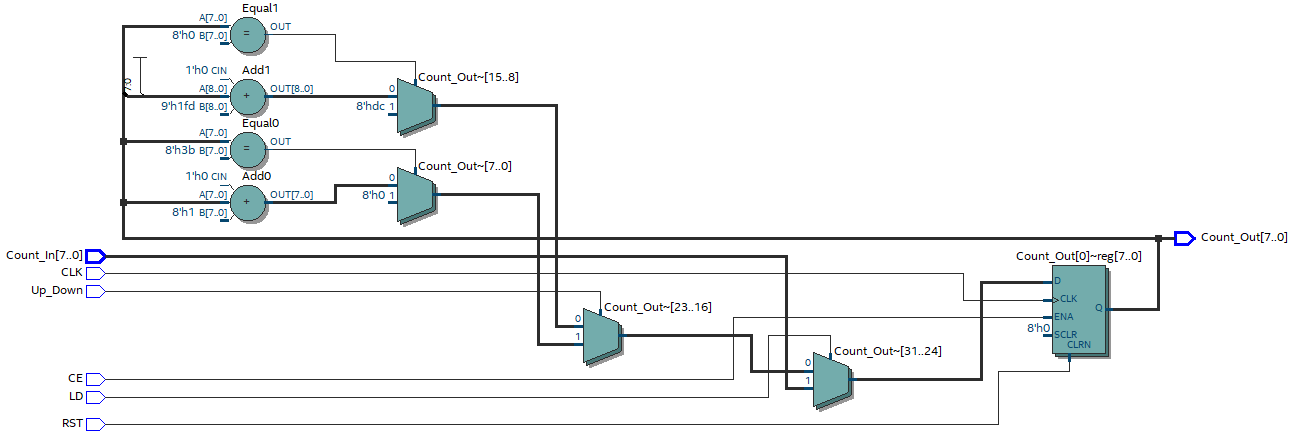
\includegraphics[scale=0.5]{Counter_Full_RTL.png}
	\caption{Diagrama RTL del contador completo de 8 bits. \label{fig:counter_full_rtl}}
\end{figure}

\begin{figure}[ht]
	\centering
	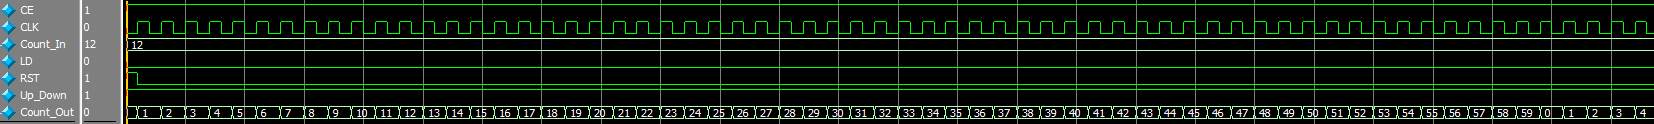
\includegraphics[scale=0.38]{Counter_Full_Wave.png}
	\caption{Simulación del contador completo de 8 bits en el visor de formas de onda de ModelSim. \label{fig:counter_full_wave}}
\end{figure}

\begin{figure}[ht]
	\centering
	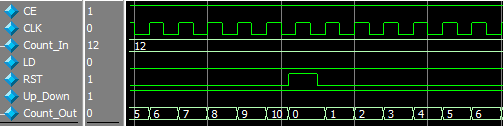
\includegraphics[scale=1.2]{Counter_Full_WaveRST.png}
	\caption {Funcionamiento del \textit{reset} asíncrono, implementado en el contador completo de 8 bits. \label{fig:counter_full_waverst}}
\end{figure}

\begin{figure}[ht]
	\centering
	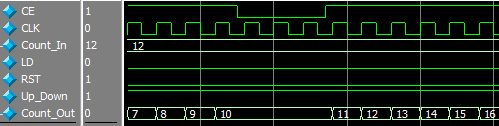
\includegraphics[scale=1.2]{Counter_Full_WaveCE.png}
	\caption{Funcionamiento del \textit{clock enable}, implementado en el contador completo de 8 bits. \label{fig:counter_full_wavece}}
\end{figure}

\begin{figure}[ht]
	\centering
	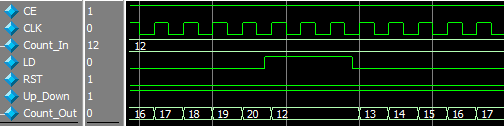
\includegraphics[scale=1.2]{Counter_Full_WaveLD.png}
	\caption{Funcionamiento de la carga de datos a la entrada, implementada en el contador completo de 8 bits. \label{fig:counter_full_waveld}}
\end{figure}

\begin{figure}[ht]
	\centering
	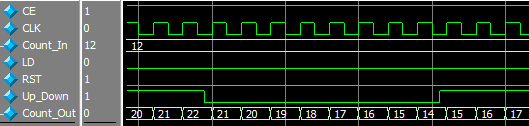
\includegraphics[scale=1.2]{Counter_Full_WaveUpDown.png}
	\caption{Funcionamiento del sentido de la cuenta, implementada en el contador completo de 8 bits. \label{fig:counter_full_waveupdown}}
\end{figure}

\begin{figure}[ht]
	\centering
	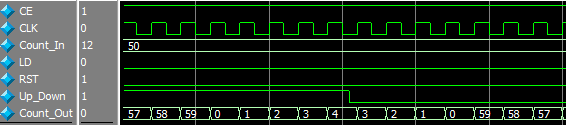
\includegraphics[scale=1.1]{Counter_Full_WaveTope.png}
	\caption{Funcionamiento del tope en la cuenta, implementado en el contador completo de 8 bits. \label{fig:counter_full_wavetope}}
\end{figure}